\chapter{Introduction}
\section{Background}

\label{sec:background}

\lettrine[findent=2pt]{\textbf{W}}{}rite some intro here. How to cite a figure. It is shown in Figure~\ref{fig:testimage}.
\begin{figure}[!h]
	\centering
	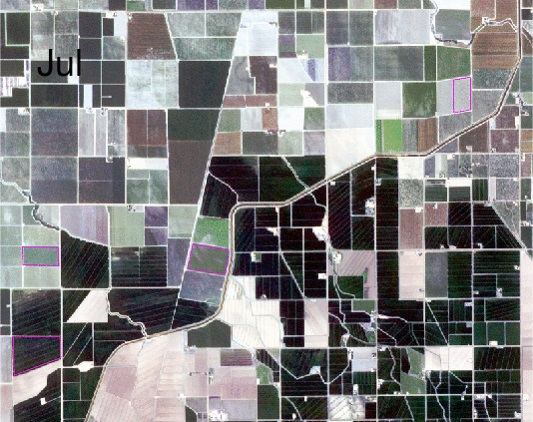
\includegraphics[width=1.0\textwidth]{Figures/testimage.jpg}
	\hspace{1mm}
	\caption{Test image include graphix.} 
	\label{fig:testimage}
\end{figure}

Snow is classified as wet or dry depending upon the amount of liquid water content. Dry snow consists of ice particles and air, whereas wet snow contains liquid water as a third component. Microwaves strongly respond to this change in liquid water content in snow~\citep{hallikainen1986dielectric}. The estimation of snowpack parameters requires a good understanding of the scattering mechanisms from the snowpack. Scattering from the air-snow surface and the uppermost layers are effective for wet snow estimation. The attenuation of a propagating EM wave is given in terms of the volume extinction coefficient ($\kappa_e$) and the penetration depth is defined as, $\delta_{p}=1/\kappa_e$. 



\section{Motivation}
\begin{itemize}
	\item SAR polarimetry is a very active research area in radar remote sensing in which there is an increased need to explore the potential for quantitative estimation of bio-/geo-physical parameters.
	
	\item Many works have reported the study of snow parameters using SAR data, among which very few studies barely attempted to retrieve any quantitative (for example snow wetness, snow density, snow grain size etc.) information.
	
	\item There is no proven precise methodology for the estimation of snowpack parameters using full polarimetric SAR data over the Indian Himalayan region. 
	
	\item The data obtained from the new generation advanced full-polarimetric SAR sensors along with the advanced polarimetric decomposition techniques, provide an opportunity to develop improved algorithms for snow pack parameters estimation. 
	
\end{itemize}
\section{Research objectives}
In this thesis, polarimetric SAR data is used for the estimation of snowpack parameters over the Indian Himalayan region. In this context algorithms have been developed for the estimation of snow wetness, snow surface dielectric constant and density,
\begin{description}
	\item[$\mbox{1(a)}.$ ] Estimation of snow wetness from dual polarimetric $(\mbox{HH}+\mbox{VV})$ coherent X-band data.
	\item[$\mbox{1(b)}.$ ] Estimation of snow wetness from full polarimetric $(\mbox{HH}+\mbox{HV}+\mbox{VH}+\mbox{VV})$ SAR data.
	\item[$\mbox{1(c)}.$ ] Estimation of snow surface dielectric constant from full polarimetric $(\mbox{HH}+\mbox{HV}+\mbox{VH}+\mbox{VV})$ SAR data.
	\item[$\mbox{2}.   $ ] Estimation of snow density from full polarimetric $(\mbox{HH}+\mbox{HV}+\mbox{VH}+\mbox{VV})$ C-band SAR data.
\end{description}

%\begin{enumerate}
%	
%\item Development of an algorithm for 
%	\begin{enumerate}
%	  \item Estimation of snow wetness from dual polarimetric $(\mbox{HH}+\mbox{VV})$ coherent TerraSAR-X X-band (9.65 GHz) data.
%	  \item Estimation of effective snowpack wetness from full polarimetric $(\mbox{HH}+\mbox{HV}+\mbox{VH}+\mbox{VV})$ Radarsat-2 (5.4 GHz) data.
%	  \item Estimation of snow surface dielectric constant from full polarimetric $(\mbox{HH}+\mbox{HV}+\mbox{VH}+\mbox{VV})$ SAR data.
%	\end{enumerate} 
%\item Development of an algorithm for estimation of snow density from full polarimetric $(\mbox{HH}+\mbox{HV}+\mbox{VH}+\mbox{VV})$ Radarsat-2 (5.4 GHz) data.
%\end{enumerate} 

These objectives are accomplished and implemented over the Indian Himalayan region for which data is acquired over the study area and field measurements were recorded during January to March 2012-2014. In the Indian Himalayan region, snowfall normally occurs during December to March from an altitude of 2000 m above the mean sea level. The expected snow wetness during Jan.-- Feb. is around 2--6 $\%$ by volume because of fresh snowfall and average minimum temperature. The snow density variation mainly depends on the temperature which produces the snow melt-freeze cycle. In the Indian Himalayan region, the mean minimum temperature in the month of January is around -15$^\circ$C-0$^\circ$C and the mean maximum temperature in the month of June is around 20$^\circ$C-30$^\circ$C. The mean high and low temperatures in the month of February over the study area are around 11$^\circ$C  and -1$^\circ$C respectively.
	  
\section{Thesis outline}
	The subject matter of the thesis is presented in the following five chapters, 
\begin{enumerate}[label=\checkmark]
\item	Chapter-1 gives an overview of the advantages of polarimetric SAR systems for snowpack parameters estimation. It also describes an outline of the snowpack parameters and their characteristics with respect to the electromagnetic waves, and also emphasizes the motivation of this research and objectives.
\item	Chapter-2 elucidates the principle and important parameters of a SAR system and the characteristics of snowpack parameters. Thorough investigations of snowpack characterization studies, PolSAR decomposition techniques and their advancements are included in this chapter. 
\item	Chapter 3 describes all the new developments of methodologies for the estimation of snow parameters from available SAR systems in separate subsections. All the new developments are presented with detailed flowcharts and derivations. The detailed description about the study area, in-situ field data collection and the data sets used for this study are incorporated in this chapter. 
\item Chapter-4 discusses the results obtained from all the algorithms and are presented in separate subsections along with detailed investigations using topographic and observatory measurements. Multi-temporal analyses of the results is also included in this chapter. 
\item	Chapter-5 highlights the new findings obtained by the utilization of SAR polarimetric data and conclusions arising out of this complete study are elucidated. The scope for future and continuation of this research work are also reported.  
%a new algorithm for the estimation of another important snowpack parameter, snow density is proposed using SAR polarimetry data. The detailed methodology with flow chart, snow density maps, thorough analysis of multi temporal variation of snow density within a season and the validation of the results are included in this section. 
%\item In Chapter-6, the proposed methodologies and the discussions of the results, including the important findings of the studies are summarized. The future scopes of the research works are proposed successively, following the conclusion on the basis of important extracts and understanding of the subject of interest.
\end{enumerate}

